\documentclass[a4paper, 12pt]{mcshw}
\begin{document}
\Letsmaketitle{8}
\begin{enumerate}
    \item Read in a photo and convert to a matrix. Perform a singular value decomposition of the matrix. Reconstruct the photo using only 10\%, 25\%, 50\% of the singular values.
        \begin{enumerate}
            \item Print the reconstructed photo. How good is the quality of the reconstructed photos?
                \begin{center}
                    \vspace{3mm}
                    \includegraphics[height=4cm]{a.bmp}
                    \includegraphics[height=4cm]{50.bmp}

                    \includegraphics[height=4cm]{25.bmp}
                    \includegraphics[height=4cm]{10.bmp}
                    \vspace{3mm}
                \end{center}
                From top to bottom, left to right, are the original picture, 50\%, 25\%, 10\% pictures.

                As we can see, the 50\% compresion performs quite well, 25\% performs a little bit noisy, while 10\% has a lot of noisy points.
                \vspace{4mm}
            \item What percent of the Forbenius norm is captured in each case.

                \vspace{2mm}
                Since I use SVD for the R, G, B matrices seperately, I captured Forbenius norm seperately too. 
                
                There are 99.9617\% for R, 99.9617\% for G, 99.9617\% for B, captured in the 50\% quality picture. 
                
                There are 99.7215\% for R, 99.7574\% for G, 99.7197\% for B, captured in the 25\% quality picture.
                
                There are 99.0076\% for R, 99.1092\% for G, 98.9815\% for B, captured in the 10\% quality picture.
        \end{enumerate}
    \item Consider the pairwise distance matrix for twenty US cities given below. Use the algorithm of Exercise 4.30 to place the cities on a map of the US. Suppose you had airline distances for 50 cities around the world. Could ou use these distances to construct a world map?
        \begin{solution}
            Let $X$ be a $20 \times 2$ matrix, Since we have
            $$(XX^T)_{ij} = -\frac{1}{2}[d_{ij}^2 - \frac{1}{n}\sum_{j = 1}^{n}d_{ij}^2 - \frac{1}{n}\sum_{i = 1}^nd_{ij}^2 + \frac{1}{n}\sum_{i = 1}^n\sum_{j = 1}^nd_{ij}^2]$$
            We can easily get $XX^T$, using singular value decomposition, we can get $XX^T = UDV^T$. Notice that the columns of $U$ are the right singular vectors of $(XX^T)^T = XX^T$, which means $U^T = V^T$, thus $U = V$.  Then we get $$XX^T = VDV^T$$ $$X = \sqrt{D}V$$ where $\sqrt{D}$ means take the square root of each element in the diagonal of $D$. The rows of $X$ are the coodinates of the cities.
            
            See the map below.
            \pagebreak
                \begin{center}
                    \fbox{
                    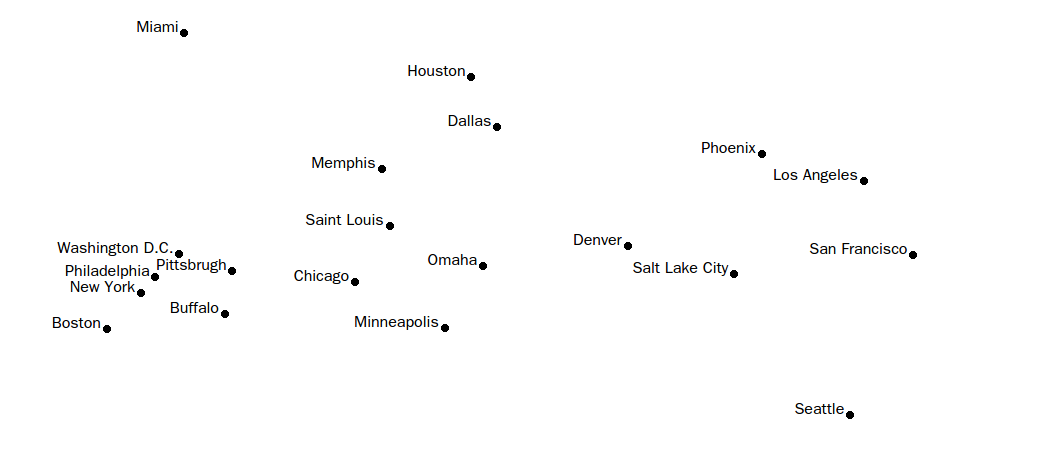
\includegraphics[height=6cm]{map.png}
                }
                \end{center}
                However we cannot use the airline distance around the world to build the map, since the earch is a sphere, not a plane.
        \end{solution}
\end{enumerate}
\end{document}
